\begin{frame}
\frametitle{Optimization of spin-coherence time \textcolor{PineGreen}{\cite{PhysRevLett.117.054801}}}
\framesubtitle{}

Precise adjustments of three sextupole families in the ring

\begin{columns}[]
	\column{0.53\textwidth}
	\begin{figure}
		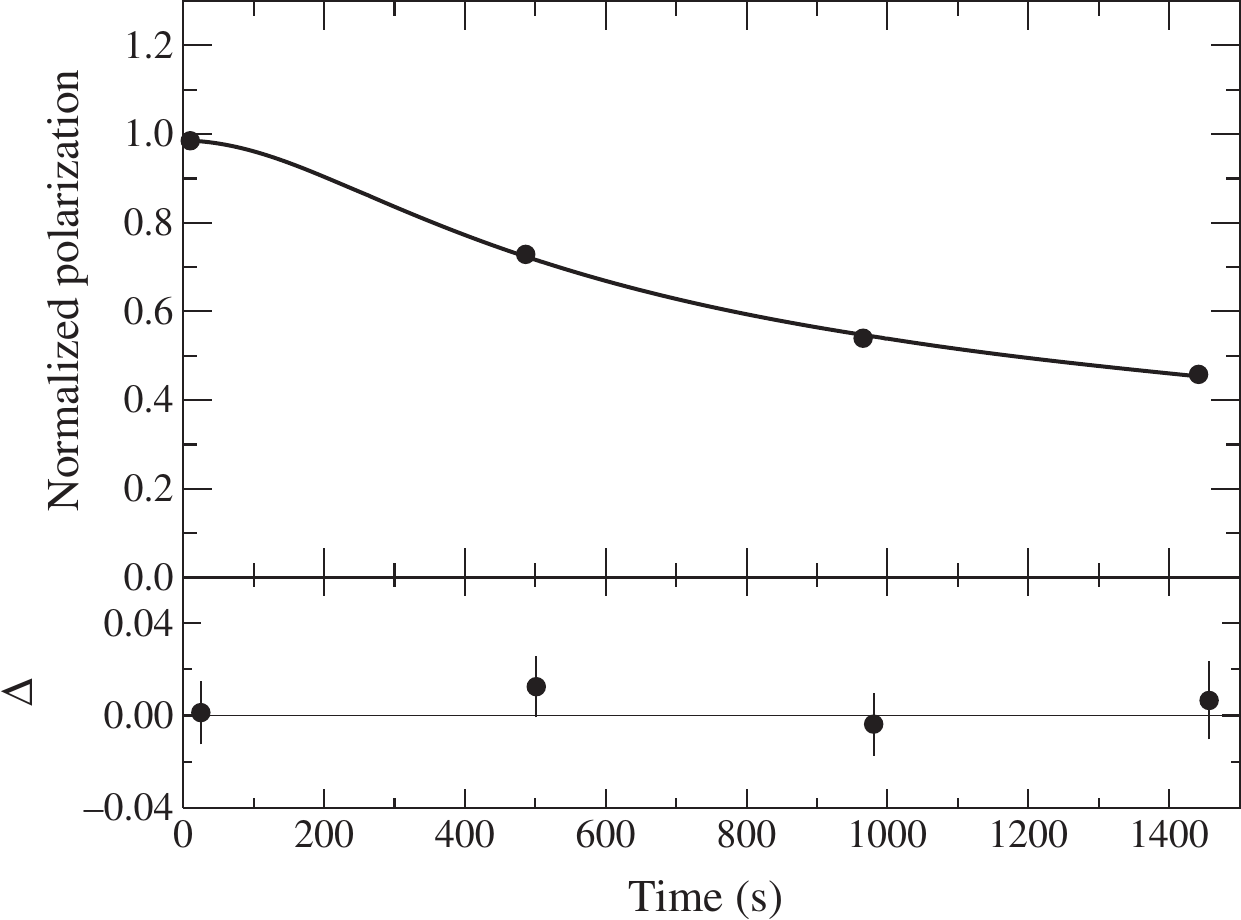
\includegraphics[width=0.95\textwidth]{spin-coherence-time-from-PRL.png}
	\end{figure}
	\column{0.4\textwidth}
	\begin{block}{JEDI progress on $\tau_\text{SCT}$:}
		\begin{equation}
		\textcolor{red}{\mathbf{\tau_\text{SCT} = (782 \pm 117)\,\text{s}}} \nonumber
		\end{equation}
		\vspace{-0.5cm}
		\begin{itemize}
			\item Previous record: $\tau_\text{SCT}(\text{VEPP}) \approx \SI{0.5}{s}$\,\textcolor{PineGreen}{\cite{Vasserman1987302}} ($\approx \num{e7}$ spin revolutions).
		\end{itemize}
	\end{block}
\end{columns}

\begin{alertblock}{\textbf{Spring 2015:} Way beyond anybody’s expectation:}
	\begin{itemize}
		\item With about $\num{e9}$ stored deuterons.
		\item Long spin coherence time was one of main obstacles of srEDM experiments.
		\item Large value of $\tau_\text{SCT}$ of crucial importance (\ref{eq:statistical-error-EDM-experiment}), since $ \sigma_\text{stat} \propto {\tau_\text{SCT}}^{-1}$.
	\end{itemize}
\end{alertblock}

\end{frame}
